
% The \phantomsection command is needed to create a link to a place in the document that is not a
% figure, equation, table, section, subsection, chapter, etc.
% https://tex.stackexchange.com/questions/44088/when-do-i-need-to-invoke-phantomsection
\phantomsection

\chapter{Integer Programming}\label{chap:integer-programming}


Integer Programming (IP), a subset of mathematical programming, addresses optimization problems where decision variables are required to take on integer values.
Specifically, mixed-integer linear programming (MILP) extends this concept by encompassing the assumption that for each possible discrete decision, a (continuous) linear program has to be solved.
The complexity of MILP problems often necessitates sophisticated solution methods to find optimal or near-optimal solutions.
This chapter provides an overview of MILP problem-solving techniques, ranging from exact methods like the branch-and-bound algorithm to approaches to provide approximate solutions, such as heuristics and matheuristics.
Through these methodologies, the groundwork is laid for the subsequent discussion on deep learning-based primal heuristics, which aim to enhance the efficiency of MILP problem solving.

\section{Integer and Combinatorial Optimization}

A solution for an integer and combinatorial optimization problem is the maximum or minimum value of a multivariate function that respects a series of inequality and equality constraints and integrality restrictions on some or all variables~\cite{nemhauserIntegerCombinatorialOptimization1999}.
It is not difficult to see that integer and combinatorial optimization encompasses a wide range of problems of practical utility.
Examples include train scheduling, airline crew scheduling, production planning, electricity generation planning, and cutting problems~\cite{wolseyIntegerProgramming1998}.

Mathematical programming is a language naturally suitable to formulate integer and combinatorial optimization problems, for example, in the form
\begin{equation}\label{eq:general-ip}\tag{IP}
    \begin{split}
	\min_{\bm{x}} \quad & f\left( \bm{x} \right) \\
	\textrm{s.t.} \quad & \bm{g}\left( \bm{x} \right) \le \bm{0} \\
	  & \bm{x} \in \Z^{n}\times \R^{p}
    ,\end{split}
\end{equation}
with $n$ integer variables and $p$ continuous variables.
Furthermore, $\bm{g}: \Z^{n}\times \R^{p} \longrightarrow \R^{m}$,  and $\bm{0}$ is a null vector of dimension $m$.
Note that maximizing a function is equivalent to minimizing its negative, and an equality constraint can be represented by two inequalities, which renders \eqref{eq:general-ip} a complete formulation.

For an integer program formulated as in \eqref{eq:general-ip}, the set \[
X=\left\{ \bm{x}\in \Z^{n}\times \R^{p}: \bm{g}\left( \bm{x} \right) \le \bm{0}\right\} 
\] is named the \emph{feasible region} of the problem, and a vector $\bm{x}\in X$ is a \emph{feasible solution}.
A feasible solution $\bm{x}^{*}\in X$ is \emph{optimal} if, and only if, there is no other feasible solution results in a lower value of the \emph{objective function} $f: \Z^{n}\times \R^{p} \longrightarrow \R$, i.e., $\bm{x}^{*}$ is optimal $\iff f(\bm{x}^{*}) \le f(\bm{x}) ,\,\forall \bm{x}\in X$.

Note that even if a problem is feasible ($X\neq \varnothing$), it may not have an optimal solution, e.g., if the feasible region is unbounded and the objective function has no global minimum.
Furthermore, if an optimal solution exists, it may no be unique.
% TODO: show how a problem may have no optimal solution even if with bounded feasible region. see Nemhauser, I.4.6

Beyond the practical applications of integer programming, its computational complexity renders it an important theoretical model.
It is easy to see that integer programming is an NP-complete problem~\cite{nemhauserIntegerCombinatorialOptimization1999}.
In fact, one of Karp's 21 NP-complete problems~\cite{karpReducibilityCombinatorialProblems1972} is a special case of integer programming with no objective function (constraint satisfaction problem) and solely binary variables.

\section{Mixed-Integer Linear Programs}

MILP is a subset of IP in which the objective and the constraints are all linear functions and the problem requires integer and continuous variables.
Formally, an MILP can be formulated as 
\begin{equation}\label{eq:general-milp}\tag{MILP}
\begin{split}
    \min_{\bm{x}} \quad & \bm{c}^{T}\bm{x} \\
    \textrm{s.t.} \quad & A\bm{x} \le \bm{b} \\
	  & \bm{x} \in \Z^{n}\times \R^{p}
,\end{split}
\end{equation}
where $A\in \R^{m\times (n+p)}$ is the constraint matrix, $\bm{b}\in \R^{m}$ is the right-hand side vector, and $\bm{c}\in \R^{n+p}$ is the cost vector.
An \emph{instance} of an MILP problem is specified by a tuple  $\left( \bm{c},\bm{b},A,n \right)$.

The significance of this class of problems has already been recognized by \citeonline{dantzigSignificanceSolvingLinear1960}.
Many well-known problems can be formulated through MILP, such as the Traveling Salesperson Problem (TSP) and the map coloring problem.
Furthermore, continuous nonlinear functions can be approximated to arbitrary quality by piecewise linear functions, which admit an MILP formulation~\cite{camponogaraModelsAlgorithmsOptimal2015}.
In other words, MILP is a powerful tool for approximating optimization problems with continuous nonlinearities.

\section{Solving MILP Problems}

% TODO: solving MILP is hard, in fact, it is NP-complete, as seen Karp's 
Although MILP offers powerful models for a wide range of problems, solving such problems is unarguably hard.
In fact, the NP-complete problem formulated by \citeonline{karpReducibilityCombinatorialProblems1972} only contains linear terms, which renders it an special case of MILP and, thus, assuming P$\neq$NP, classifies MILP problems as NP-complete.
However, despite the intractable nature, there are efficient and reliable algorithms and software solutions for the computation of optimal and approximate solutions to MILP problems~\cite{bengioMachineLearningCombinatorial2021}.
Furthermore, the applications of MILP often require high-quality solutions in a limited time, which motivate the development of heuristic approaches, i.e., approaches that trade optimality (or feasibility) guarantees for a tractable running time.

\subsection{The Branch-and-Bound Algorithm}

The branch-and-bound algorithm follows a divide-and-conquer approach.
An MILP problem is divided into smaller, easier problems, and the solution to these problems is combined such that a solution to the original problem is found~\cite{wolseyIntegerProgramming1998}.

An MILP problem is divided by decomposing its feasible region.
Given a problem $P$ as in \eqref{eq:general-milp} with feasible region $X=\{\bm{x}\in \Z^{n}\times \R^{p}: A\bm{x}\le \bm{b}\}$, a decomposition of its feasible region $X_1,\ldots,X_K$ is such that $X=X_1\cup \ldots\cup X_K$.
In this context, a subproblem is
\begin{equation}\label{eq:milp-subproblem}
\begin{split}
    P^{(k)} : \min_{\bm{x}} \quad & \bm{c}^{T}\bm{x} \\
    \textrm{s.t.} \quad & \bm{x}\in X_k
,\end{split}
\end{equation}
for which $\bm{x}^{k}$ is the optimal solution and $z^{k}=\bm{c}^{T}\bm{x}^{k}$ is the optimal cost.
If the $k$-th subproblem is infeasible, it is assumed that $z^{k}=\infty$.
If $k^{*}= \arg\min_k z^{k}$, then $z^{k^*}$ is the optimal value of the MILP problem $P$ and $\bm{x}^{k^*}$ is its optimal solution.

A decomposition is useful for a divide-and-conquer approach if the resulting subproblems are significantly easier to solve than the original problem.
One way to achieve this is by decomposing the feasible region on the values for the integer variables.
If this decomposition strategy is performed recursively until all integer variables have only one feasible assignment in each $X_k$, then each $P^{(k)}$ is an LP problem, which allows us to compute, for each $k$ the optimal solution in polynomial time.
For example, consider an MILP problem with 3 binary variables, i.e., with $X\subseteq \{0,1\}^{3}\times \R^{p}$.
By recursively decomposing $X$ on the possible assignments for each binary variable, the tree structure of Fig.~\ref{fig:binary-MILP-tree-example} could be assembled.
% Note that a decomposition can be progressively generated by exploring the tree, e.g., $X=X_1\cup X_2\cup X_3\cup X_4$, $X=X_1\cup X_2\cup X_3\cup X_{4, 1}\cup X_{4,2}$, \ldots, $X=X_{1,1}\cup X_{1,2}\cup X_{2,1}\cup \ldots\cup X_{4,2}$.
% Note that $X_{1,2}$ and $X_{4,2}$ are empty sets, i.e., the associated subproblems are infeasible.

\begin{figure}[h]
    \centering
    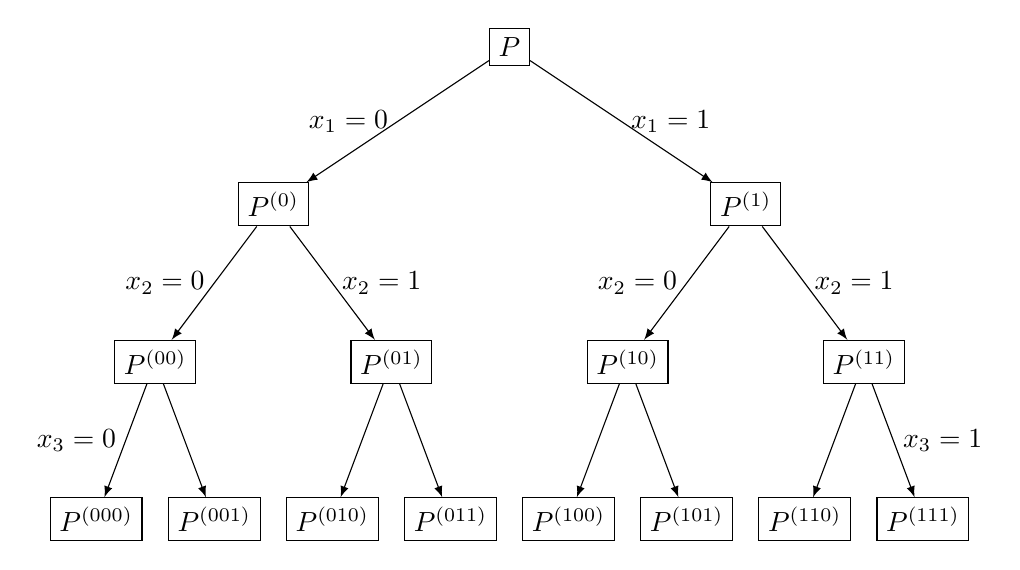
\begin{tikzpicture}[every child node/.style={rectangle,draw},level 1/.style={sibling distance=6cm},level 2/.style={sibling distance=3cm},level 3/.style={sibling distance=1.5cm}, level distance = 2cm,edge from parent/.style={draw,-latex}]
        \node[rectangle,draw] (X) {$P$} 
	    child { node {$P^{(0)}$}
        	child { node {$P^{(00)}$}
		    child { node {$P^{(000)}$} edge from parent node [midway,left] {$x_3=0$} }
		    child { node {$P^{(001)}$} }
		    edge from parent node [midway,left] {$x_2=0$}
		}
        	child { node {$P^{(01)}$}
		    child { node {$P^{(010)}$} }
		    child { node {$P^{(011)}$} }
		    edge from parent node [midway,right] {$x_2=1$}
		}
        	edge from parent node [midway,left] {$x_1=0$}
            }
            child { node {$P^{(1)}$}
        	child { node {$P^{(10)}$}
		    child { node {$P^{(100)}$} }
		    child { node {$P^{(101)}$} }
		    edge from parent node [midway,left] {$x_2=0$}
		}
        	child { node {$P^{(11)}$}
		    child { node {$P^{(110)}$} edge from parent }
		    child { node {$P^{(111)}$} edge from parent node [midway,right] {$x_3=1$} }
		    edge from parent node [midway,right] {$x_2=1$}
		}
        	edge from parent node [midway,right] {$x_1=1$}
            }
            ;
	%\node[left = of x2] (x2_label) {$x_2=$};
	%\node at (x2_label |- x1) {$x_1=$};
	% \node[left = of x1 -| x2] {$x_1=$};
    \end{tikzpicture}
    \caption{Complete decomposition of an MILP problem on its 3 binary variables. Nodes are annotated with the associated subproblems. Assuming that the problem has no other integer variables, the subproblems at the leaf nodes are LP problems.}
    \label{fig:binary-MILP-tree-example}
\end{figure}

Unfortunately, completely decomposing an MILP problem through the integer variable assignments is only possible for very small, bounded problems.
If the problem is unbounded in the integer variables, the complete decomposition would result in an infinite recursion.
Furthermore, the number of leaf nodes grows exponentially with the size of the problem\footnotemark.
\footnotetext{In this context, the size of the problem is measured as the number of binary variables that the equivalent reformulation as a binary MILP would contain. The number of leaf nodes grows exponentially (with base 2) with respect to the number of such binary variables.}

The branch-and-bound algorithm follows an implicit approach that uses upper and lower bounds to avoid indefinitely dividing subsets from the decomposition.
Let $P$ be an MILP problem formulated as in \eqref{eq:general-milp} and $X_1,\ldots,X_K$ be a decomposition of the feasible region $X$.
If $\underline{z}^{k}$ and $\overline{z}^{k}$ are lower and upper bounds to $z^{k}$ (optimum cost of $P^{(k)}$), for every $k=1,\ldots,K$, then, it is true that \[
\min_k \underline{z}^{k} \le z \le \min_k \overline{z}^{k}
,\] 
where $z$ is the optimum cost of $P$.
In other words, we can compute bounds of the root problem as $\underline{z}\gets \min_k \underline{z}^{k}$ and $\overline{z}\gets \min_k \overline{z}^{k}$.
Finally, if $\underline{z}^{k} \ge \overline{z}$ for a given $k$, then the optimal solution of $P^{(k)}$ will not be an optimal solution of $P$, because it is guaranteed that another subproblem has a better feasible solution.
In other words, even if the optimal solution of $P^{(k)}$ is unknown, it is possible to disregard $X_k$ in the decomposition, i.e., $X_k$ does not need to be further subdivided. 

For example, let $P$ be an MILP problem and $X=X_1\cup X_2$ be a decomposition such that $X_1=\{\bm{x}\in X: x_1 \le 2\}$ and $X_2=\{\bm{x}\in X: x_1 \ge 3\}$.
Suppose that the LP relaxations\footnote{The linear programming problem obtained by ignoring the integrality constraints of an MILP is called its \emph{LP relaxation}.} of $P^{(1)}$ and $P^{(2)}$ were solved to optimality, giving lower bounds $\underline{z}^1=20$ and $\underline{z}^{2}=15$, and that a feasible solution to $P$ is known in $X_2$ such that the upper bound $\overline{z}^{2}=17$ is known.
Fig.~\ref{fig:pruning-example-milp} illustrates the decomposition along with respective bounds in the form of a tree.
Because the lower bound of $P^{(1)}$ is greater than the original problem's upper bound (as $\overline{z}=\min_k \overline{z}^{k}$), the optimal solution is definitely not in $X_1$, so this set is ignored in the decomposition and not further refined.

\begin{figure}[h]
    \centering
    \begin{tikzpicture}[every child node/.style={rectangle,draw},level 1/.style={sibling distance=3cm}, level distance = 2cm,edge from parent/.style={draw,-latex}]
        \node[rectangle,draw] (P) {$P$} 
	    child { node[fill=red!50] (P1) {$P^{(1)}$}
        	edge from parent node [midway,left] (x1) {$x_1\le 2$}
            }
            child { node (P2) {$P^{(2)}$}
        	edge from parent node [midway,right] {$x_1 \ge 3$}
            }
            ;
	%\node[above = 0cm of P] {$15\le z\le 17$} ;
	\node[right = 0.5cm of P.south] {$15$} ;
	\node[right = 0.5cm of P.north] {$17$} ;
	\node[right = 0.5cm of P1.south] {$20$} ;
	\node[right = 0.5cm of P2.north] {$17$} ;
	\node[right = 0.5cm of P2.south] {$15$} ;
	%\node[left = of x2] (x2_label) {$x_2=$};
	%\node at (x2_label |- x1) {$x_1=$};
	% \node[left = of x1 -| x2] {$x_1=$};
    \end{tikzpicture}
    \caption{Example of pruning the decomposition of an MILP problem based on known bounds. The lower (resp. upper) bounds of each (sub)problem are annotated at the bottom (resp. top) right of each node. The node associated to set $X_1$ is painted red to indicate it is pruned based on the bounds of the root problem, which are updated based on the bounds from $P^{(2)}$.}
    \label{fig:pruning-example-milp}
\end{figure}

Because of the usual tree representation, the operation of disregarding a set in the decomposition is often called \emph{pruning}.
3 basic rules can be listed that lead to pruning of the branch associated to set $X_k$:
\begin{itemize}
    \item[Optimality] Subproblem $P^{(k)}$ was solved to optimality (e.g., through its LP relaxation having an optimal solution that respects the integrality constraints);
    \item[Bound] The associated lower bound is higher than the upper bound of the root problem ($\underline{z}^{k}\ge \overline{z}$);
    \item[Infeasibility] $X_k = \varnothing$.
\end{itemize}


The two key components of a branch-and-bound algorithm are the pruning system based on \emph{bounds}, as discussed above, and the rules for subdividing the sets in the decomposition, or \emph{branching}.
A simple strategy for branching is to choose an integer variable that has taken a fractional value in the optimal solution to the LP relaxation and split the problem on this factional value.
For example, let $X_k$ be a set in the decomposition of an MILP problem, and $P^{(k)}$ be the associated subproblem.
Let $\widetilde{\bm{x}}^{k}$ be the solution to the LP relaxation of $P^{(k)}$, and suppose that the integer variable $x_3$ takes value $3.67$ in $\widetilde{\bm{x}}^{k}$.
Following the proposed branching strategy on $x_3$, the sets $X_{k_1}$ and $X_{k_2}$ would be created such that \[
X_{k_1} = \left\{ \bm{x} \in X_k : x_3 \le 3 \right\} ,\, X_{k_2} = \left\{ \bm{x}\in X_k : x_3 \ge 4 \right\} 
,\] and the set $X_k$ would then be replaced in the decomposition by these two new sets.
Fig.~\ref{fig:branching-example} illustrates this example.

\begin{figure}[h]
    \centering
    \begin{tikzpicture}[every child node/.style={rectangle,draw},level 1/.style={sibling distance=3cm}, level distance = 2cm,edge from parent/.style={draw,-latex}]
        \node (P) {} 
	    child { node[draw=none] (P1) {}
        	edge from parent [draw=none]
            }
            child { node (Pk) {$P^{(k)}$}
		child { node [solid] (Pk1) {$P^{(k_1)}$}
		    edge from parent [solid] node [midway,left] (x1) {$x_3\le 3$}
		}
		child { node [solid] (Pk2) {$P^{(k_2)}$}
		    edge from parent [solid] node [midway,right] (x2) {$x_3\ge 4$}
		}
        	edge from parent [dashed] 
            }
            ;
	\node[right = 0cm of Pk.east] {$\widetilde{x}^{k}_3 = 3.67$} ;
    \end{tikzpicture}
    \caption{Example of branching on a given set $X_k$ which composes the decomposition of an MILP problem. Only the relevant part of the tree is illustrated (indicated by the dashed arrow). The optimum value of $x_3$ (the selected integer variable for branching) in the LP relaxation of $P^{(k)}$ is annotated next to the appropriated node.}
    \label{fig:branching-example}
\end{figure}

Note that by branching on the fractional value of an integer variable in the optimal solution to the LP relaxation, the optimal solution of the LP relaxation becomes infeasible in the LP relaxations of the new sets\footnote{This is true unless there are degeneracies such as multiple solutions in the LP relaxation}.
Therefore, after branching, the best lower bound will necessarily increase.
Using the example above to make this result tangible, it is possible to state that $\widetilde{\bm{x}}^{k}$ is infeasible for the LP relaxations of both $P^{(k_1)}$ and $P^{(k_2)}$.
Therefore, $\max\{\underline{z}^{k_1},\underline{z}^{k_2}\} > \underline{z}^{k}$.

%As an example, take the MILP problem\footnote{Example taken from \citeonline{vanderbeiLinearProgrammingFoundations1998}, Ch. 22.5.}
%\begin{align*}
%    \min_{\bm{x}} \quad & -17 x_1 - 12x_2 \\
%    \textrm{s.t.} \quad & 10x_1 + 7x_2 \le 40 \\
%      & x_1+x_2\le 5 \\
%      & \bm{x} \in \Z_+^2
%.\end{align*}

There are many more intricate details to the construction of a branch-and-bound algorithm, such as the strategy for choosing a set in the decomposition to refine, the amount of information from each node of the tree to be stored, efficient reoptimization, and computing the bounds using the dual.
The reader is pointed to \citeonline{wolseyIntegerProgramming1998} and \citeonline{vanderbeiLinearProgrammingFoundations1998} for advanced topics and detailed examples.


\subsection{Heuristics}


\subsection{Matheuristics}



